\documentclass[12pt]{article}

%------------- PREAMBLE -------------
\usepackage[margin=1in]{geometry}
\usepackage{amsmath,amssymb,mathtools}
\usepackage{enumitem}
\usepackage{bm}
\usepackage{hyperref}
\usepackage{fancyhdr}
\usepackage{draftwatermark}
\usepackage{xcolor}
\usepackage{titlesec}
\usepackage{tikz}
\usetikzlibrary{arrows.meta,calc,positioning}

%------------- TITLE AND METADATA -------------
\newcommand{\CourseCode}{MH1301}
\newcommand{\CourseName}{Discrete Mathematics}
\newcommand{\DocType}{Tutorial 10}

\title{
\CourseCode\ \CourseName \\[0.3em]
\large \DocType
}
\author{
  Academic Year 2025/2026, Semester 2 \\[0.25em]
  \textit{Quantitative Research Society @NTU}
}
\date{\today}

%------------- HEADER & FOOTER (for page 2 onward) -------------
\fancypagestyle{main}{
  \fancyhf{}
  \fancyhead[L]{\CourseCode\ \CourseName}
  \fancyhead[R]{\href{https://qrsntu.org}{QRS@NTU}}
  \fancyfoot[C]{\thepage}
  \renewcommand{\headrulewidth}{0.4pt}
  \renewcommand{\footrulewidth}{0pt}
}

%------------- SIMPLE FOOTER (page 1 only) -------------
\fancypagestyle{plainfirst}{
  \fancyhf{}
  \renewcommand{\headrulewidth}{0pt}
  \renewcommand{\footrulewidth}{0pt}
  \fancyfoot[C]{\scriptsize\textcolor{gray}{\textit{For academic reference only. This document is provided for educational purposes and does not constitute an official question paper, answer key, or any formally authorised academic material. Its content is not guaranteed to be complete or accurate.}}}
}

%------------- WATERMARK -------------
\SetWatermarkText{Unofficial --- QRS@NTU --- qrsntu.org}
\SetWatermarkScale{1}
\SetWatermarkLightness{0.985}

%------------- SHORTCUTS -------------
\newcommand{\N}{\mathbb{N}}
\newcommand{\Z}{\mathbb{Z}}
\newcommand{\R}{\mathbb{R}}
\newcommand{\comp}[1]{\overline{#1}}
\newcommand{\V}{V}
\newcommand{\E}{E}
\newcommand{\degG}{\deg}
\newcommand{\diam}{\operatorname{diam}}

\DeclareMathOperator{\dist}{dist}

\tikzset{
  vtx/.style={circle, draw, minimum size=20pt, inner sep=1pt},
  dotv/.style={circle, fill, inner sep=1.5pt},
  smallv/.style={circle, fill, inner sep=1.25pt},
  every picture/.style={line cap=round, line join=round}
}

\setcounter{secnumdepth}{-1}
\setcounter{tocdepth}{3}
\setlist[enumerate]{itemsep=0.3em, topsep=0.3em}
\setlist[itemize]{itemsep=0.2em, topsep=0.2em}
\setlength{\headheight}{14.5pt}

\begin{document}

%------------- COVER PAGE -------------
\maketitle
\thispagestyle{plainfirst}
\pagestyle{main}

%====================================================
% OVERVIEW
%====================================================
\begin{center}
  \rule{0.82\textwidth}{0.4pt}\\[4pt]
  \textbf{Overview}\\[2pt]
  \rule{0.82\textwidth}{0.4pt}
\end{center}

\noindent
This tutorial focuses on planar graph bounds, bipartite planar graphs, regular planar graphs, and chromatic numbers of wheel graphs. The main tools are:
\begin{itemize}[leftmargin=*]
  \item Euler's formula for connected planar graphs;
  \item planar edge bounds for simple planar and bipartite planar graphs;
  \item degree counting via the Handshake Lemma;
  \item complement edge counting;
  \item wheel graphs and chromatic-number parity;
  \item bipartite graphs and odd-cycle obstructions;
  \item explicit planar constructions and non-planarity by density.
\end{itemize}

\noindent
\textbf{Question map.}
\begin{itemize}[leftmargin=*]
  \item Question 1: Euler's formula, face degrees, and girth bounds.
  \item Question 2: planarity of $K_{2,n}$ and nonexistence of planar $6$-regular simple graphs.
  \item Question 3: complement edge counting and unavoidable non-planarity.
  \item Question 4: planar cubic examples and planar edge upper bounds.
  \item Question 5: chromatic numbers of wheel graphs.
  \item Question 6: degree-$1$ graphs and $2$-colourability.
  \item Question 7: adding edges to wheel graphs.
  \item Question 8: possible numbers of regions in connected planar graphs.
  \item Question 9: bipartite planar region bounds and a $6$-vertex $8$-region example.
\end{itemize}

\newpage
\tableofcontents
\newpage

%====================================================
% QUESTION 1
%====================================================
\section{Question 1 (Euler formula and face-degree bounds)}

\subsection{Problem}
\begin{enumerate}[label=(\alph*)]
  \item Suppose that a connected planar graph has eight vertices, each of degree three. Into how many regions is the plane divided by a planar representation of this graph?
  \item Suppose that a connected planar simple graph with $m$ edges and $n$ vertices contains no simple circuits of length $4$ or less. Show that
  \[
    m\le \frac{5}{3}n-\frac{10}{3}
  \]
  if $n\ge 4$.
\end{enumerate}

\subsection{Solution}

\subsubsection{Method 1: Euler formula and direct face-degree counting}
\begin{enumerate}[label=(\alph*)]
  \item \textbf{Theorem/criterion used.} For a connected planar graph with $n$ vertices, $m$ edges, and $r$ regions,
  \[
    n-m+r=2.
  \]
  Also, the Handshake Lemma gives
  \[
    \sum_{v\in V}\deg(v)=2m.
  \]

  Here $n=8$, and every vertex has degree $3$. Hence
  \[
    2m=8\cdot 3=24,
    \qquad
    m=12.
  \]
  By Euler's formula,
  \[
    8-12+r=2.
  \]
  Therefore
  \[
    r=6.
  \]
  Thus
  \[
    \boxed{6}
  \]
  regions are formed.

  \item Since the graph has no simple circuit of length $4$ or less, every face boundary has length at least $5$. Let $\deg(R)$ denote the number of edge-sides on the boundary of a region $R$, with a bridge counted twice if it appears twice in a boundary walk. Then
  \[
    \sum_R \deg(R)=2m.
  \]
  Since every region has degree at least $5$,
  \[
    2m=\sum_R \deg(R)\ge 5r.
  \]
  Hence
  \[
    r\le \frac{2m}{5}.
  \]
  By Euler's formula,
  \[
    r=m-n+2.
  \]
  Thus
  \[
    m-n+2\le \frac{2m}{5}.
  \]
  Multiplying by $5$ gives
  \[
    5m-5n+10\le 2m.
  \]
  Therefore
  \[
    3m\le 5n-10,
  \]
  and hence
  \[
    \boxed{m\le \frac{5}{3}n-\frac{10}{3}.}
  \]
\end{enumerate}

\subsubsection{Method 2: Planar girth inequality}
\textbf{Theorem/criterion used.} If a connected simple planar graph has girth at least $g\ge 3$, then
\[
  m\le \frac{g}{g-2}(n-2).
\]
This follows from
\[
  2m=\sum_R\deg(R)\ge gr
\]
and Euler's formula $r=m-n+2$.

\begin{enumerate}[label=(\alph*)]
  \item The graph is $3$-regular on $8$ vertices. Hence
  \[
    m=\frac{3\cdot 8}{2}=12.
  \]
  Euler's formula gives
  \[
    r=2-n+m=2-8+12=6.
  \]
  Therefore
  \[
    \boxed{r=6.}
  \]

  \item The hypothesis says that the graph has no cycle of length $3$ or $4$. Hence its girth is at least $5$. Apply the planar girth inequality with $g=5$:
  \[
    m\le \frac{5}{5-2}(n-2)
    =\frac{5}{3}(n-2)
    =\frac{5}{3}n-\frac{10}{3}.
  \]
  Thus
  \[
    \boxed{m\le \frac{5}{3}n-\frac{10}{3}.}
  \]
\end{enumerate}

%====================================================
% QUESTION 2
%====================================================
\newpage
\section{Question 2 (Planarity of $K_{2,n}$ and planar $6$-regular graphs)}

\subsection{Problem}
\begin{enumerate}[label=(\alph*)]
  \item Prove that $K_{2,5}$ is planar by drawing the graph without edges that cross each other. What about $K_{2,n}$?
  \item Prove that there are no $6$-regular simple graphs that are planar. \textit{(Hint: How many edges does a $6$-regular graph have?)}
\end{enumerate}

\subsection{Solution}

\subsubsection{Method 1: Explicit drawing and planar edge bound}
\begin{enumerate}[label=(\alph*)]
  \item The graph $K_{2,5}$ has bipartition
  \[
    \{l_1,l_2\}\sqcup \{r_1,r_2,r_3,r_4,r_5\}.
  \]
  A planar drawing is:
  \begin{center}
  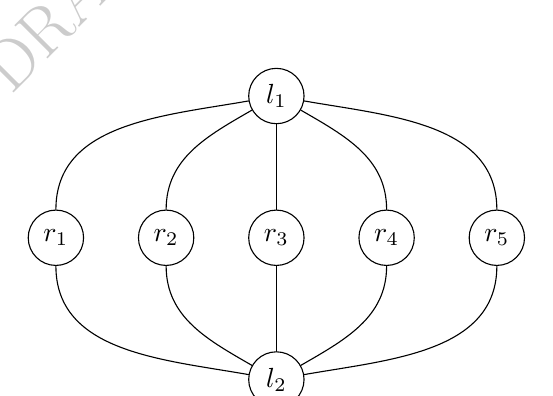
\begin{tikzpicture}[scale=1.0]
    \node[vtx] (l1) at (0,1.8) {$l_1$};
    \node[vtx] (l2) at (0,-1.8) {$l_2$};

    \node[vtx] (r1) at (-2.8,0) {$r_1$};
    \node[vtx] (r2) at (-1.4,0) {$r_2$};
    \node[vtx] (r3) at (0,0) {$r_3$};
    \node[vtx] (r4) at (1.4,0) {$r_4$};
    \node[vtx] (r5) at (2.8,0) {$r_5$};

    \draw (l1) to[out=190,in=90] (r1);
    \draw (l1) to[out=210,in=90] (r2);
    \draw (l1)--(r3);
    \draw (l1) to[out=-30,in=90] (r4);
    \draw (l1) to[out=-10,in=90] (r5);

    \draw (l2) to[out=170,in=-90] (r1);
    \draw (l2) to[out=150,in=-90] (r2);
    \draw (l2)--(r3);
    \draw (l2) to[out=30,in=-90] (r4);
    \draw (l2) to[out=10,in=-90] (r5);
  \end{tikzpicture}
  \end{center}
  This drawing has no crossing edges.

  More generally, $K_{2,n}$ is planar for every $n\ge 1$: place the $n$ vertices $r_1,\dots,r_n$ on a horizontal line, place $l_1$ above the line and $l_2$ below the line, draw all $l_1r_i$ edges in the upper half-plane, and draw all $l_2r_i$ edges in the lower half-plane. No two edges cross except at common endpoints. Hence
  \[
    \boxed{K_{2,n}\text{ is planar for every }n\ge 1.}
  \]

  \item \textbf{Theorem/criterion used.} A simple planar graph with $n\ge 3$ vertices and $m$ edges satisfies
  \[
    m\le 3n-6.
  \]

  If a graph is $6$-regular on $n$ vertices, then the Handshake Lemma gives
  \[
    2m=\sum_{v\in V}\deg(v)=6n.
  \]
  Hence
  \[
    m=3n.
  \]
  But a planar simple graph must satisfy
  \[
    m\le 3n-6<3n.
  \]
  This contradicts $m=3n$. Therefore
  \[
    \boxed{\text{there is no planar simple }6\text{-regular graph}.}
  \]
\end{enumerate}

\subsubsection{Method 2: General construction and average-degree obstruction}
\begin{enumerate}[label=(\alph*)]
  \item For $K_{2,n}$, write the bipartition as
  \[
    L=\{u,v\},
    \qquad
    R=\{x_1,\dots,x_n\}.
  \]
  Put $x_1,\dots,x_n$ in order on a line, draw $u$ above and $v$ below. Draw all edges $ux_i$ using pairwise noncrossing arcs above the line, and all edges $vx_i$ using pairwise noncrossing arcs below the line. Since upper and lower arcs lie in disjoint half-planes, no crossing is produced. Hence
  \[
    \boxed{K_{2,n}\text{ is planar}.}
  \]

  \item \textbf{Theorem/criterion used.} Every simple planar graph has average degree strictly less than $6$. Indeed, from $m\le 3n-6$,
  \[
    \frac{1}{n}\sum_{v\in V}\deg(v)=\frac{2m}{n}\le \frac{2(3n-6)}{n}=6-\frac{12}{n}<6.
  \]
  A $6$-regular graph has average degree exactly $6$. This contradicts the strict planar average-degree bound. Therefore
  \[
    \boxed{\text{no }6\text{-regular simple graph is planar}.}
  \]
\end{enumerate}

%====================================================
% QUESTION 3
%====================================================
\newpage
\section{Question 3 (A graph or its complement must be nonplanar)}

\subsection{Problem}
Show that if $G$ is a simple graph with at least $11$ vertices, then either $G$ or $\comp{G}$, the complement of $G$, is nonplanar.

\subsection{Solution}

\subsubsection{Method 1: Add the two planar edge bounds}
\textbf{Theorem/criterion used.} If a simple planar graph has $n\ge 3$ vertices and $m$ edges, then
\[
  m\le 3n-6.
\]
Also, for a simple graph $G$ on $n$ vertices,
\[
  |E(G)|+|E(\comp{G})|=\binom{n}{2}.
\]

Suppose, for contradiction, that both $G$ and $\comp{G}$ are planar. Let
\[
  m=|E(G)|.
\]
Then
\[
  |E(\comp{G})|=\binom{n}{2}-m.
\]
Since both graphs are planar,
\[
  m\le 3n-6
\]
and
\[
  \binom{n}{2}-m\le 3n-6.
\]
Adding,
\[
  \binom{n}{2}\le 6n-12.
\]
Thus
\[
  \frac{n(n-1)}{2}\le 6n-12.
\]
Multiplying by $2$,
\[
  n(n-1)\le 12n-24,
\]
so
\[
  n^2-13n+24\le 0.
\]
But for $n\ge 11$,
\[
  n^2-13n+24
  =n(n-13)+24.
\]
At $n=11$ this equals
\[
  121-143+24=2>0,
\]
and the quadratic is increasing for all $n\ge 11$. Hence the inequality is impossible for $n\ge 11$.

Therefore the assumption that both $G$ and $\comp{G}$ are planar is false. Thus
\[
  \boxed{\text{for }n\ge 11,\text{ at least one of }G\text{ and }\comp{G}\text{ is nonplanar}.}
\]

\subsubsection{Method 2: Pigeonhole density argument}
\textbf{Theorem/criterion used.} A simple planar graph on $n\ge 3$ vertices has at most $3n-6$ edges.

Since
\[
  |E(G)|+|E(\comp{G})|=\binom{n}{2},
\]
at least one of $G,\comp{G}$ has at least half of the total number of possible edges:
\[
  \max\{|E(G)|,|E(\comp{G})|\}\ge \frac{1}{2}\binom{n}{2}
  =\frac{n(n-1)}{4}.
\]
For $n\ge 11$,
\[
  \frac{n(n-1)}{4}>3n-6.
\]
Indeed,
\[
  \frac{n(n-1)}{4}>3n-6
  \iff
  n^2-n>12n-24
  \iff
  n^2-13n+24>0,
\]
which holds for every integer $n\ge 11$.

Thus at least one of $G$ and $\comp{G}$ has more than $3n-6$ edges. Such a graph cannot be planar. Hence
\[
  \boxed{\text{either }G\text{ or }\comp{G}\text{ is nonplanar}.}
\]

%====================================================
% QUESTION 4
%====================================================
\newpage
\section{Question 4 (Planar cubic examples and edge upper bounds)}

\subsection{Problem}
\begin{enumerate}[label=(\alph*)]
  \item Find a planar $3$-regular graph.
  \item Is there a planar graph with $10$ vertices and $25$ edges?
\end{enumerate}

\subsection{Solution}

\subsubsection{Method 1: $K_4$ example and Euler edge bound}
\begin{enumerate}[label=(\alph*)]
  \item Take
  \[
    G=K_4.
  \]
  A planar drawing is:
  \begin{center}
  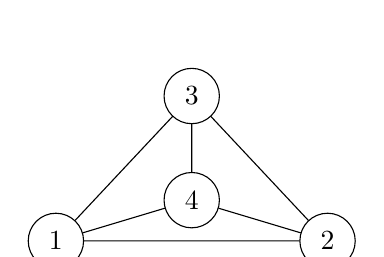
\begin{tikzpicture}[scale=1.15]
    \node[vtx] (1) at (-1.5,0) {$1$};
    \node[vtx] (2) at (1.5,0) {$2$};
    \node[vtx] (3) at (0,1.6) {$3$};
    \node[vtx] (4) at (0,0.45) {$4$};
    \draw (1)--(2)--(3)--(1);
    \draw (4)--(1) (4)--(2) (4)--(3);
  \end{tikzpicture}
  \end{center}
  Since every vertex of $K_4$ is adjacent to the other three vertices,
  \[
    \deg(v)=3
    \qquad
    \text{for all }v\in V(K_4).
  \]
  Hence $K_4$ is planar and $3$-regular. Therefore
  \[
    \boxed{K_4\text{ is a planar }3\text{-regular graph}.}
  \]

  \item \textbf{Theorem/criterion used.} A simple planar graph with $n\ge 3$ vertices and $m$ edges satisfies
  \[
    m\le 3n-6.
  \]
  For $n=10$,
  \[
    m\le 3(10)-6=24.
  \]
  A graph with $10$ vertices and $25$ edges would have
  \[
    25>24,
  \]
  contradicting the planar edge bound. Therefore
  \[
    \boxed{\text{there is no planar simple graph with }10\text{ vertices and }25\text{ edges}.}
  \]
\end{enumerate}

\subsubsection{Method 2: Tetrahedral graph and maximal-planar obstruction}
\begin{enumerate}[label=(\alph*)]
  \item The tetrahedral graph is the graph of a tetrahedron. Its graph is exactly $K_4$. It has four vertices and every vertex is incident to the three other vertices. Thus it is $3$-regular. Since it is the edge graph of a convex polyhedron, it has a planar representation. Hence
  \[
    \boxed{K_4\text{ works}.}
  \]

  \item A maximal simple planar graph on $n\ge 3$ vertices triangulates the sphere and has exactly
  \[
    3n-6
  \]
  edges. Therefore no simple planar graph on $10$ vertices can have more than
  \[
    3(10)-6=24
  \]
  edges. Since $25>24$,
  \[
    \boxed{\text{no such planar graph exists}.}
  \]
\end{enumerate}

%====================================================
% QUESTION 5
%====================================================
\newpage
\section{Question 5 (Chromatic numbers of wheel graphs)}

\subsection{Problem}
Determine the chromatic numbers of the following three graphs, called wheel graphs.

\begin{center}
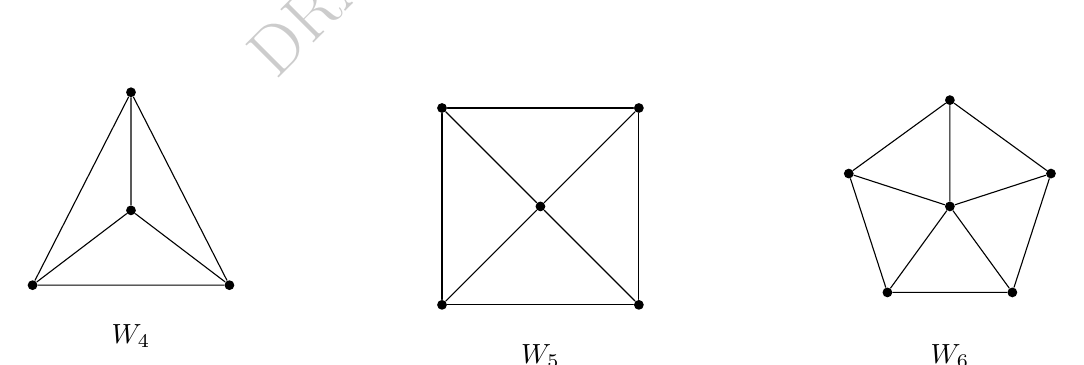
\begin{tikzpicture}[scale=1.0]
  % W4
  \begin{scope}[shift={(-5.2,0)}]
    \node[smallv,label=above:{}] (t) at (0,1.45) {};
    \node[smallv] (l) at (-1.25,-1.0) {};
    \node[smallv] (r) at (1.25,-1.0) {};
    \node[smallv] (c) at (0,-0.05) {};
    \draw (t)--(l)--(r)--(t);
    \draw (c)--(t) (c)--(l) (c)--(r);
    \node at (0,-1.65) {$W_4$};
  \end{scope}

  % W5
  \begin{scope}[shift={(0,0)}]
    \node[smallv] (tl) at (-1.25,1.25) {};
    \node[smallv] (tr) at (1.25,1.25) {};
    \node[smallv] (br) at (1.25,-1.25) {};
    \node[smallv] (bl) at (-1.25,-1.25) {};
    \node[smallv] (cc) at (0,0) {};
    \draw (tl)--(tr)--(br)--(bl)--(tl);
    \draw (cc)--(tl) (cc)--(tr) (cc)--(br) (cc)--(bl);
    \node at (0,-1.9) {$W_5$};
  \end{scope}

  % W6
  \begin{scope}[shift={(5.2,0)}]
    \node[smallv] (v1) at (90:1.35) {};
    \node[smallv] (v2) at (18:1.35) {};
    \node[smallv] (v3) at (-54:1.35) {};
    \node[smallv] (v4) at (-126:1.35) {};
    \node[smallv] (v5) at (162:1.35) {};
    \node[smallv] (h) at (0,0) {};
    \draw (v1)--(v2)--(v3)--(v4)--(v5)--(v1);
    \draw (h)--(v1) (h)--(v2) (h)--(v3) (h)--(v4) (h)--(v5);
    \node at (0,-1.9) {$W_6$};
  \end{scope}
\end{tikzpicture}
\end{center}

\subsection{Solution}

\subsubsection{Method 1: Wheel graph formula from rim parity}
\textbf{Definition used.} In this tutorial's notation, $W_n$ is obtained by taking a cycle
\[
  C_{n-1}
\]
and adding one central vertex adjacent to every vertex of the cycle.

The central vertex is adjacent to every rim vertex, so its colour cannot be used on the rim. Hence
\[
  \chi(W_n)=\chi(C_{n-1})+1.
\]
For cycles,
\[
  \chi(C_k)=
  \begin{cases}
  2, & k\text{ even},\\
  3, & k\text{ odd}.
  \end{cases}
\]

For $W_4$, the rim is $C_3$, so
\[
  \chi(W_4)=\chi(C_3)+1=3+1=4.
\]

For $W_5$, the rim is $C_4$, so
\[
  \chi(W_5)=\chi(C_4)+1=2+1=3.
\]

For $W_6$, the rim is $C_5$, so
\[
  \chi(W_6)=\chi(C_5)+1=3+1=4.
\]

Therefore
\[
  \boxed{\chi(W_4)=4,\qquad \chi(W_5)=3,\qquad \chi(W_6)=4.}
\]

\subsubsection{Method 2: Lower bounds and explicit colourings}
\begin{enumerate}[label=(\alph*)]
  \item For $W_4$, the graph is $K_4$: the rim is a triangle and the centre is adjacent to all three rim vertices. Since every pair of vertices is adjacent,
  \[
    \chi(W_4)=4.
  \]
  Thus
  \[
    \boxed{\chi(W_4)=4.}
  \]

  \item For $W_5$, the rim is $C_4$. Colour the four rim vertices alternately with colours $1$ and $2$. The centre is adjacent to every rim vertex, so it must receive a third colour. Hence
  \[
    \chi(W_5)\le 3.
  \]
  Also, $W_5$ contains a triangle formed by the centre and any rim edge, so
  \[
    \chi(W_5)\ge 3.
  \]
  Therefore
  \[
    \boxed{\chi(W_5)=3.}
  \]

  \item For $W_6$, the rim is $C_5$, an odd cycle. Thus the rim already requires three colours:
  \[
    \chi(C_5)=3.
  \]
  The centre is adjacent to every rim vertex. In any proper colouring of $C_5$, all three colours appear on the rim. Hence the centre cannot use any of those three colours, so
  \[
    \chi(W_6)\ge 4.
  \]
  Four colours suffice by using three colours on the rim and a fourth colour on the centre. Hence
  \[
    \boxed{\chi(W_6)=4.}
  \]
\end{enumerate}

%====================================================
% QUESTION 6
%====================================================
\newpage
\section{Question 6 (Degree-one graphs and two-colourability)}

\subsection{Problem}
\begin{enumerate}[label=(\alph*)]
  \item Under what condition on $n$ is there a graph with $n$ vertices where all vertices have degree $1$?
  \item True or false: a planar graph that has no subgraph that is an odd cycle can be $2$-colored.
\end{enumerate}

\subsection{Solution}

\subsubsection{Method 1: Handshake Lemma and bipartite criterion}
\begin{enumerate}[label=(\alph*)]
  \item If all $n$ vertices have degree $1$, then
  \[
    \sum_{v\in V}\deg(v)=n.
  \]
  By the Handshake Lemma, the sum of all degrees must equal $2m$, so it must be even. Hence $n$ must be even.

  Conversely, if $n$ is even and $n\ge 2$, pair the vertices:
  \[
    \{v_1,v_2\},\{v_3,v_4\},\dots,\{v_{n-1},v_n\},
  \]
  and add the edges
  \[
    v_1v_2,\ v_3v_4,\ \dots,\ v_{n-1}v_n.
  \]
  This gives a disjoint union of $\frac n2$ copies of $K_2$, and every vertex has degree $1$.

  Therefore
  \[
    \boxed{\text{such a graph exists exactly when }n\ge 2\text{ is even}.}
  \]

  \item \textbf{Theorem/criterion used.} A graph is bipartite if and only if it has no odd cycle. A graph is $2$-colourable if and only if it is bipartite.

  The graph has no subgraph that is an odd cycle, so it has no odd cycle. Therefore it is bipartite, and hence it can be coloured with two colours. Planarity is not needed.

  Thus the statement is
  \[
    \boxed{\text{True}.}
  \]
\end{enumerate}

\subsubsection{Method 2: Matching construction and BFS colouring}
\begin{enumerate}[label=(\alph*)]
  \item A graph in which every vertex has degree $1$ is a perfect matching: every component is a single edge $K_2$. Hence the vertices are partitioned into pairs. Such a partition exists precisely when $n$ is even. For ordinary positive vertex counts, this gives
  \[
    \boxed{n\text{ even and }n\ge 2.}
  \]

  \item Assume the graph has no odd cycle. In each connected component, choose a root vertex and colour each vertex by the parity of its distance from the root:
  \[
    \text{colour }0\text{ if }\dist(r,v)\text{ is even},
    \qquad
    \text{colour }1\text{ if }\dist(r,v)\text{ is odd}.
  \]
  If an edge joined two vertices of the same parity level, then the two shortest root paths together with that edge would produce an odd cycle. This is impossible. Hence every edge joins vertices of opposite colours.

  Therefore the graph is $2$-colourable, so the statement is
  \[
    \boxed{\text{True}.}
  \]
\end{enumerate}

%====================================================
% QUESTION 7
%====================================================
\newpage
\section{Question 7 (Adding edges to wheel graphs)}

\subsection{Problem}
\begin{enumerate}[label=(\alph*)]
  \item How many edges does one have to add to the wheel graph $W_5$ so that the resulting simple graph is non-planar?
  \item If we add three new edges to $W_6$ so that the result is a simple graph, can the result be planar?
\end{enumerate}

\subsection{Solution}

\subsubsection{Method 1: Completion to $K_5$ and planar edge bound}
\begin{enumerate}[label=(\alph*)]
  \item The wheel graph $W_5$ has $5$ vertices. It consists of a $4$-cycle and a centre adjacent to all four rim vertices, so
  \[
    |E(W_5)|=4+4=8.
  \]
  The complete graph $K_5$ has
  \[
    \binom{5}{2}=10
  \]
  edges. Therefore $W_5$ is missing exactly
  \[
    10-8=2
  \]
  edges from $K_5$.

  Adding these two missing edges produces $K_5$, which is nonplanar. Adding only one edge gives a $5$-vertex graph with $9$ edges. Since $K_5-e$ is planar, one edge is not enough to force non-planarity from $W_5$; the resulting graph is a subgraph of $K_5-e$ up to isomorphism and remains planar.

  Therefore
  \[
    \boxed{2}
  \]
  edges are needed.

  \item The wheel graph $W_6$ has a $5$-cycle as its rim and one central vertex. Hence
  \[
    |E(W_6)|=5+5=10.
  \]
  Adding three new edges gives a simple graph with
  \[
    m=10+3=13
  \]
  edges and
  \[
    n=6
  \]
  vertices.

  A simple planar graph with $6$ vertices has at most
  \[
    3n-6=3(6)-6=12
  \]
  edges. Since
  \[
    13>12,
  \]
  the resulting graph cannot be planar. Hence
  \[
    \boxed{\text{No}.}
  \]
\end{enumerate}

\subsubsection{Method 2: Kuratowski-minimal obstruction and density}
\begin{enumerate}[label=(\alph*)]
  \item \textbf{Theorem/criterion used.} The smallest simple nonplanar graph on five vertices is $K_5$. Equivalently, every proper subgraph of $K_5$ is planar.

  The graph $W_5$ has $5$ vertices and is missing exactly the two diagonals of the outer $4$-cycle. Adding both missing edges yields $K_5$, so two edges are sufficient. With only one added edge, the graph is still a proper subgraph of $K_5$, hence planar. Therefore
  \[
    \boxed{2\text{ edges are necessary and sufficient}.}
  \]

  \item A planar simple graph on $6$ vertices has at most $12$ edges. The graph obtained from $W_6$ by adding three new simple edges has $13$ edges. Hence it violates the planar edge bound and cannot be planar:
  \[
    \boxed{\text{No, the result cannot be planar}.}
  \]
\end{enumerate}

%====================================================
% QUESTION 8
%====================================================
\newpage
\section{Question 8 (Connected planar graphs with prescribed number of regions)}

\subsection{Problem}
\begin{enumerate}[label=(\alph*)]
  \item Is there a connected planar graph with $n$ vertices and $2n$ regions?
  \item Is there a connected planar graph with $n$ vertices and $n$ regions?
\end{enumerate}

\subsection{Solution}

\subsubsection{Method 1: Euler formula and wheel construction}
\begin{enumerate}[label=(\alph*)]
  \item \textbf{Theorem/criterion used.} A simple planar graph with $n\ge 3$ vertices and $m$ edges satisfies
  \[
    m\le 3n-6.
  \]
  For a connected planar graph,
  \[
    r=m-n+2.
  \]
  Hence
  \[
    r\le (3n-6)-n+2=2n-4.
  \]
  Since
  \[
    2n>2n-4,
  \]
  a connected simple planar graph cannot have $2n$ regions. Therefore
  \[
    \boxed{\text{No}.}
  \]

  \item Yes. For $n\ge 4$, take the wheel graph $W_n$. It has $n$ vertices: one central vertex and a rim cycle on $n-1$ vertices. Its number of edges is
  \[
    m=(n-1)+(n-1)=2n-2.
  \]
  Since $W_n$ is connected and planar, Euler's formula gives
  \[
    r=m-n+2=(2n-2)-n+2=n.
  \]
  Hence
  \[
    \boxed{\text{Yes, }W_n\text{ is an example for }n\ge 4.}
  \]
\end{enumerate}

\subsubsection{Method 2: Maximal-planar bound and triangulated wheel faces}
\begin{enumerate}[label=(\alph*)]
  \item In a simple connected planar graph, the maximum number of regions occurs when the graph is maximal planar. In that case,
  \[
    m=3n-6
  \]
  and hence
  \[
    r=m-n+2=3n-6-n+2=2n-4.
  \]
  Thus no simple connected planar graph can reach $2n$ regions. Therefore
  \[
    \boxed{\text{No connected simple planar graph has }2n\text{ regions}.}
  \]

  \item The wheel graph $W_n$ has a rim cycle of length $n-1$ and one hub. Its planar drawing has:
  \begin{itemize}[leftmargin=*]
    \item $n-1$ triangular regions incident with the hub;
    \item one exterior region bounded by the rim cycle.
  \end{itemize}
  Therefore the total number of regions is
  \[
    (n-1)+1=n.
  \]
  Hence
  \[
    \boxed{\text{Yes, }W_n\text{ gives }n\text{ vertices and }n\text{ regions}.}
  \]
\end{enumerate}

%====================================================
% QUESTION 9
%====================================================
\newpage
\section{Question 9 (Bipartite planar region bounds and a six-vertex example)}

\subsection{Problem}
\begin{enumerate}[label=(\alph*)]
  \item Let $n\ge 3$. Is there a connected, planar, bipartite graph with $n$ regions and $n$ vertices?
  \item Is there a connected planar graph with $6$ vertices and $8$ regions?
\end{enumerate}

\subsection{Solution}

\subsubsection{Method 1: Bipartite planar edge bound and octahedral construction}
\begin{enumerate}[label=(\alph*)]
  \item \textbf{Theorem/criterion used.} A connected simple bipartite planar graph with $n\ge 3$ vertices and $m$ edges satisfies
  \[
    m\le 2n-4.
  \]
  This follows because every face has boundary length at least $4$, so
  \[
    2m=\sum_R\deg(R)\ge 4r,
  \]
  and Euler's formula gives the bound.

  If such a graph had $n$ vertices and $n$ regions, then by Euler's formula,
  \[
    n-m+n=2.
  \]
  Hence
  \[
    m=2n-2.
  \]
  But the bipartite planar edge bound gives
  \[
    m\le 2n-4.
  \]
  These two equations would imply
  \[
    2n-2\le 2n-4,
  \]
  impossible. Therefore
  \[
    \boxed{\text{No such connected planar bipartite graph exists}.}
  \]

  \item Yes. Take the octahedral graph. It has $6$ vertices and $12$ edges. A planar drawing is:
  \begin{center}
  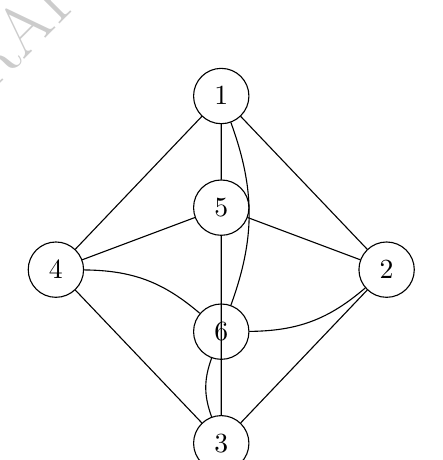
\begin{tikzpicture}[scale=1.05]
    \node[vtx] (T) at (0,2.1) {$1$};
    \node[vtx] (R) at (2.0,0) {$2$};
    \node[vtx] (B) at (0,-2.1) {$3$};
    \node[vtx] (L) at (-2.0,0) {$4$};
    \node[vtx] (I) at (0,0.75) {$5$};
    \node[vtx] (O) at (0,-0.75) {$6$};

    \draw (T)--(R)--(B)--(L)--(T);
    \draw (I)--(T) (I)--(R) (I)--(B) (I)--(L);
    \draw (O) to[bend right=20] (T);
    \draw (O) to[bend right=20] (R);
    \draw (O) to[bend right=20] (B);
    \draw (O) to[bend right=20] (L);
  \end{tikzpicture}
  \end{center}
  By Euler's formula,
  \[
    r=m-n+2=12-6+2=8.
  \]
  Hence there is a connected planar graph with $6$ vertices and $8$ regions:
  \[
    \boxed{\text{Yes}.}
  \]
\end{enumerate}

\subsubsection{Method 2: Region-count contradiction and triangulated $W_6$ construction}
\begin{enumerate}[label=(\alph*)]
  \item Since the graph is bipartite, it has no odd cycle. In particular, a planar embedding has no triangular face. Hence every face has length at least $4$:
  \[
    \deg(R)\ge 4
    \qquad
    \text{for every region }R.
  \]
  Thus
  \[
    2m=\sum_R\deg(R)\ge 4r.
  \]
  If $r=n$, then
  \[
    2m\ge 4n,
    \qquad
    m\ge 2n.
  \]
  But Euler's formula with $r=n$ gives
  \[
    n-m+n=2,
    \qquad
    m=2n-2.
  \]
  Combining,
  \[
    2n-2\ge 2n,
  \]
  contradiction. Therefore
  \[
    \boxed{\text{No}.}
  \]

  \item Start with $W_6$, which has $6$ vertices and
  \[
    5+5=10
  \]
  edges. Draw $W_6$ with the hub inside the rim pentagon. Add two noncrossing diagonals in the exterior face of the rim pentagon, for example from one rim vertex to two nonadjacent rim vertices. The result is still planar and simple, and it has
  \[
    m=10+2=12
  \]
  edges.

  A schematic drawing is:
  \begin{center}
  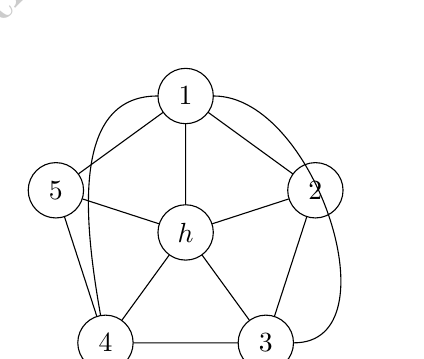
\begin{tikzpicture}[scale=1.05]
    \node[vtx] (h) at (0,0) {$h$};
    \node[vtx] (v1) at (90:1.65) {$1$};
    \node[vtx] (v2) at (18:1.65) {$2$};
    \node[vtx] (v3) at (-54:1.65) {$3$};
    \node[vtx] (v4) at (-126:1.65) {$4$};
    \node[vtx] (v5) at (162:1.65) {$5$};

    \draw (v1)--(v2)--(v3)--(v4)--(v5)--(v1);
    \draw (h)--(v1) (h)--(v2) (h)--(v3) (h)--(v4) (h)--(v5);

    \draw (v1) to[out=0,in=0] (v3);
    \draw (v1) to[out=180,in=100] (v4);
  \end{tikzpicture}
  \end{center}

  By Euler's formula,
  \[
    r=m-n+2=12-6+2=8.
  \]
  Hence
  \[
    \boxed{\text{Yes, such a graph exists}.}
  \]
\end{enumerate}

\end{document}